\chapter{Theory}
\section{Image}

In computer science, a 2d-image is defined by a function f(x,y) where (x,y) are spacial coordinate of a plane and the amplitude represent the gray level of the point.

There are many tools to work with the image. The most common is the filters. A filter is a function defined on the plane (x,y), in such way, its 2D-convolution with a image is able to extract some feature of this image. Two traditional filter are the high-pass filter, which emphasizes the lines and curve of the image, and the low-pass filter, which blur the image reducing the noise of the image.

Another tools is the transformation. The transformation take a function f, thus the image, and apply a operation that change the domain and consequentially the amplitude of the image. The goal is evidence something which was difficult to see on the original domain.

One of the most famous transformation is the Fourier transform, defined by:
\begin{equation}\label{Fourier}
F(m,n) = \int_{-\infty}^\infty{\int_{-\infty}^\infty {f(x,y)\mathrm{e}^{-2\pi\mathrm{i}(mx+ny)} \mathrm{d}x} \mathrm{d}y}
\end{equation}

Further, the Radon transform is well-know transform which has a important role in tomography.


\section{Radon transform}

The Radon transform maps a function f(x,y) into the set of all its line integrals:
\[(Rf)(l) = \int_l{f(x,y)ds}\]

Where we can parameterize $l$ as a affine function in the cartesian coordinate.
\[ R(p,q) = \int_{-\infty}^\infty {f(x,px+q) \mathrm{d}x}. \]

Sometimes is useful read the Radon transform in the polar coordinate, so:
\begin{align} 
R(\theta,x') &= \int_{-\infty}^\infty \int_{-\infty}^\infty {f(x',y') \mathrm{d}x'\mathrm{d}y'} \nonumber \\
&= \int_{-\infty}^\infty \int_{-\infty}^\infty {f(x\cos\theta+y\sin\theta,-x\sin\theta+y\cos\theta) \mathrm{d}x\mathrm{d}y } \label{Radon}
\end{align}

Where,
\[ x' =  x\cos\theta+y\sin\theta \]
\[y' =  -x\sin\theta+y\cos\theta \]

\begin{figure}[h]
\centering
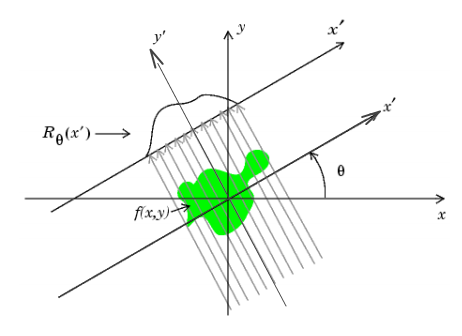
\includegraphics[scale=0.8]{img/radon_ref}
\caption{{Referential system of radon transform}}\label{radon_ref}
\end{figure}

So, we can transform a image that is in Cartesian domain to another image in radon domain using the equation \eqref{Radon}, the image in the radon domain is called sinogram. The opposite, from sinogram obtain a Cartesian image can't be done directly.

However exist another way to accomplish this task.

The inversion is done through a relationship between Fourier Transform of Radon Transform.
\[ P(\theta,k') = \int_{-\infty}^\infty { R(\theta,x')\mathrm{e}^{-2\pi\mathrm{i}k'x'} \mathrm{d}x'} \]

Using \eqref{Radon},
\[ P(\theta,k')	= \int_{-\infty}^\infty {\left({\int_{-\infty}^\infty {f(x',y')\mathrm{d}y')}}\right)\mathrm{e}^{-2\pi\mathrm{i}k'x'} \mathrm{d}x'} \]
\[ P(\theta,k') = \int_{-\infty}^\infty {\int_{-\infty}^\infty {f(x',y')\mathrm{e}^{-2\pi\mathrm{i}k'(x\cos\theta+y\sin\theta)} \mathrm{d}x'}\mathrm{d}y'} \]	
\begin{equation}\label{TCS}
P(\theta,k') = F(k'\cos\theta,k'\sin\theta)
\end{equation}

The equation \eqref{TCS}, known by theorem of the central section, says that the Fourier transform of a projection $P(\theta,k')$, is equal to the Fourier transform of $f(x,y)$ calculated along the strait line described by the angle $\theta$ with respect to k on the plane $(k,l)$.

So, if we take the Radon transform of a image F, put it on the polar coordinate, do its Fourier transform, return it to the Cartesian coordinate, and do its inverse Fourier transform, we retrieve the image F.

In theory this method work, but in practice we can't do it, because we have a finite number of projection, i.e, we have projection only for a few number of discrete angles. A ingenious procedure to resolve it, would be interpolate the missing data, although this method adds high frequency error on the reconstruct image.

Since is not recommended to do the restoration using Fourier transform, were created a alternative method which is based on the theorem of the central section. 

Starting from the Fourier transform of the image F and putting it on polar coordinate, we obtain $F(\theta, k')$. Thus, to get back the image f, the inverse Fourier transformed can be written like this.

\[ f(x,y) = \int_{-\infty}^\infty{\int_{-\infty}^\infty {F(m,n)\mathrm{e}^{2\pi\mathrm{i}(mx+ny)} \mathrm{d}m} \mathrm{d}n} \]
\[ f(x,y) = \int_{0}^{2\pi}{\int_{0}^\infty {F(k'\cos\theta,k'\sin\theta)\mathrm{e}^{2\pi\mathrm{i}k'(x \cos\theta+y\sin\theta)}k'\mathrm{d}k'} \mathrm{d}\theta} \]

Where,
\[ m = k'\cos\theta \]
 \[  l = k'\sin\theta\]

So, using the central section theorem \eqref{TCS}, we obtain
\[ f(x,y) = \int_{0}^{2\pi}{\int_{0}^\infty {P(\theta,k')\mathrm{e}^{2\pi\mathrm{i}k'(x\cos\theta+y\sin\theta)}k'\mathrm{d}k'} \mathrm{d}\theta}, \]
which can be manipulated, applying the symmetry property, arriving to
\[ f(x,y) = \int_{0}^{\pi}{\int_{-\infty}^\infty {P(\theta,k')\mathrm{e}^{2\pi\mathrm{i}k'(x\cos\theta+y\sin\theta)}|k'|\mathrm{d}k'} \mathrm{d}\theta} \]
\[ = \int_{0}^{\pi}{\int_{-\infty}^\infty {P(\theta,k')\mathrm{e}^{2\pi\mathrm{i}k'x'}|k'|\mathrm{d}k'} \mathrm{d}\theta} .\]
Thus,
\begin{equation}\label{Restore}
f(x,y) = \int_{0}^{\pi}{C(\theta,x)\mathrm{d}\theta .}
\end{equation}
Where,
\[ C(\theta,x) = \int_{-\infty}^\infty {P(\theta,k')|k'|\mathrm{e}^{2\pi\mathrm{i}k'x'}\mathrm{d}k' }\] 
and this can be interpreted as a convolution, because
\[ C(\theta,x) =  \mathrm{F}^{-1}(\mathrm{F}(R)\mathrm{F}(B)) \]
\[ B(k') = \begin{cases}  |k'| &  k'<\frac{1}{2\Delta x'}\\
                            0  & \text{otherwise}\\  \end{cases} \]
$B(k')$ is defined in this way because  we need to take in consideration the Shannon-Nyquist theorem, that specify the maximum possible frequency with respect to the number of samples, so $B(k')$ is responsible for the term $B(k')$ and to limit the frequency.

Therefore,
\begin{equation}\label{Conv}
C(\theta,x) = R(\theta,x')*B(x')
\end{equation}

Finally, the equation \eqref{Restore} show how restore image through the convolution obtained in \eqref{Conv}.

This method is called Filtered Back Projection.
